\documentclass{beamer}
\usepackage[danish]{babel}
\usetheme[width=2cm]{Hannover}
\usepackage{caption}
\captionsetup{labelformat=empty,font={scriptsize,sf}}
\usepackage[latin1]{inputenc}
\title{Savannah}
\author{sw603}
\institute{Software}
\date{26/1 - 2012}

\usepackage{epsfig}

\setbeamertemplate{blocks}[rounded]
\usepackage{color}
\usepackage{subfigure}

%LOL MARTIN!
\definecolor{darkgray}{rgb}{0.95,0.95,0.95}
\definecolor{darkgreen}{rgb}{0.00,0.50,0.00}
\usepackage{listings}
\lstset{language=Java, backgroundcolor=\color{darkgray}, basicstyle=\small, commentstyle=\color{darkgreen}, keywordstyle=\color{purple}}
\lstset{linewidth=\textwidth, showstringspaces=false}
\lstset{numbers=left, stepnumber=5, numbersep=10pt}
\lstset{frame=trBL}
\lstset{ %
language=Java,                % choose the language of the code
basicstyle=\tiny,       % the size of the fonts that are used for the code
numbers=left,                   % where to put the line-numbers
numberstyle=\tiny,      % the size of the fonts that are used for the line-numbers
stepnumber=1,                   % the step between two line-numbers. If it's 1 each line will be numbered
numbersep=5pt,                  % how far the line-numbers are from the code
backgroundcolor=\color{darkgray},  % choose the background color. You must add \usepackage{color}
showspaces=false,               % show spaces adding particular underscores
showstringspaces=false,         % underline spaces within strings
showtabs=false,                 % show tabs within strings adding particular underscores
frame=single,	                % adds a frame around the code
tabsize=2,	                % sets default tabsize to 2 spaces
captionpos=b,                   % sets the caption-position to bottom
breaklines=true,                % sets automatic line breaking
breakatwhitespace=false,        % sets if automatic breaks should only happen at whitespace
title=\lstname,                 % show the filename of files included with \lstinputlisting; also try caption instead of title
%escapeinside={\%*}{*)}          % if you want to add a comment within your code
morekeywords={*,...}            % if you want to add more keywords to the set
}
%End lool martin


%BLOCK STUFF
\makeatletter
\newcommand\beamerboxesframed[2][]{%
  \global\let\beamer@firstlineitemizeunskip=\relax%
  \vbox\bgroup%
  \setkeys{beamerboxes}{upper=block title,lower=block body,width=\textwidth}%
  \setkeys{beamerboxes}{#1}%
  {%
    \usebeamercolor{\bmb@lower}%
    \globalcolorstrue%
    \colorlet{lower.bg}{bg}%
  }%
  {%
    \usebeamercolor{\bmb@upper}%
    \globalcolorstrue%
    \colorlet{upper.bg}{bg}%
  }%
  %
  % Typeset head
  %
  \vskip4bp
  \setbox\bmb@box=\hbox{%
    \begin{minipage}[b]{\bmb@width}%
      \usebeamercolor[fg]{\bmb@upper}%
      #2%
    \end{minipage}}%
  \ifdim\wd\bmb@box=0pt%
    \setbox\bmb@box=\hbox{}%
    \ht\bmb@box=0pt%
    \bmb@prevheight=-4.5pt%
  \else%
    \wd\bmb@box=\bmb@width%
    \bmb@temp=\dp\bmb@box%
    \ifdim\bmb@temp<1.5pt%
      \bmb@temp=1.5pt%
    \fi%
    \setbox\bmb@box=\hbox{\raise\bmb@temp\hbox{\box\bmb@box}}%
    \dp\bmb@box=0pt%
    \bmb@prevheight=\ht\bmb@box%
  \fi%
  \bmb@temp=\bmb@width%
  \bmb@dima=\bmb@temp\advance\bmb@dima by2.2bp%
  \bmb@dimb=\bmb@temp\advance\bmb@dimb by4bp%
  \hbox{%
    \begin{pgfpicture}{0bp}{+-\ht\bmb@box}{0bp}{+-\ht\bmb@box}
      \ifdim\wd\bmb@box=0pt%
        \color{lower.bg}%
      \else%
        \color{upper.bg}%
      \fi%
      \pgfpathqmoveto{-4bp}{-1bp}
      \pgfpathqcurveto{-4bp}{1.2bp}{-2.2bp}{3bp}{0bp}{3bp}
      \pgfpathlineto{\pgfpoint{\bmb@temp}{3bp}}
      \pgfpathcurveto%
      {\pgfpoint{\bmb@dima}{3bp}}%
      {\pgfpoint{\bmb@dimb}{1.2bp}}%
      {\pgfpoint{\bmb@dimb}{-1bp}}%
      \bmb@dima=-\ht\bmb@box%
      \advance\bmb@dima by-2pt%
      \pgfpathlineto{\pgfpoint{\bmb@dimb}{\bmb@dima}}
      \pgfpathlineto{\pgfpoint{-4bp}{\bmb@dima}}
      \pgfpathclose
      \pgfsetstrokecolor{black}\pgfusepath{stroke, fill}
    \end{pgfpicture}%
    \copy\bmb@box%
  }%
  \nointerlineskip%
  \ifdim\wd\bmb@box=0pt
  \else
    \vskip2.4pt%
  \fi%
  \nointerlineskip%
  \setbox\bmb@colorbox=\hbox{{\pgfpicturetrue\pgfsetcolor{lower.bg}}}%
  \setbox\bmb@box=\hbox\bgroup\begin{minipage}[b]{\bmb@width}%
    \vskip2pt%
    \usebeamercolor[fg]{\bmb@lower}%
    \colorlet{beamerstructure}{upper.bg}%
    \colorlet{structure}{upper.bg}%
    %\color{.}%
}


\def\endbeamerboxesframed{%
  \end{minipage}\egroup%
  \wd\bmb@box=\bmb@width%
  \bmb@temp=\dp\bmb@box%
  \advance\bmb@temp by.5pt%
  \setbox\bmb@box=\hbox{\raise\bmb@temp\hbox{\box\bmb@box}}%
  \dp\bmb@box=0pt%
  \bmb@temp=\wd\bmb@box%
  \bmb@dima=\bmb@temp\advance\bmb@dima by2.2bp%
  \bmb@dimb=\bmb@temp\advance\bmb@dimb by4bp%
  \hbox{%
    \begin{pgfpicture}{0bp}{0bp}{0bp}{0bp}
      \unhbox\bmb@colorbox%
      \pgfpathmoveto{\pgfpoint{-4bp}{\ht\bmb@box}}
      \pgfpathlineto{\pgfpoint{-4bp}{1bp}}
      \pgfpathqcurveto{-4bp}{-1.2bp}{-2.2bp}{-3bp}{0bp}{-3bp}
      \pgfpathlineto{\pgfpoint{\the\bmb@temp}{-3bp}}
      \pgfpathcurveto%
      {\pgfpoint{\the\bmb@dima}{-3bp}}%
      {\pgfpoint{\the\bmb@dimb}{-1.2bp}}%
      {\pgfpoint{\the\bmb@dimb}{1bp}}%
      {
      \bmb@dima=\ht\bmb@box%
      \pgfpathlineto{\pgfpoint{\bmb@dimb}{\bmb@dima}}
      \pgfsetstrokecolor{black}\pgfusepath{stroke, fill}
      }
    \end{pgfpicture}%
    \box\bmb@box%
  }%
  \vskip2bp%
  \egroup% of \vbox\bgroup
}
\makeatother
\setbeamercolor{block title}{fg=black,bg=blue!30}
\setbeamercolor{block body}{fg=black,bg=blue!20}
\setbeamercolor{block title alerted}{fg=black,bg=orange!30}
\setbeamercolor{block body alerted}{fg=black,bg=orange!20}
\setbeamercolor{block title example}{fg=black,bg=green!20}
\setbeamercolor{block body example}{fg=black,bg=green!5}
\setbeamerfont{block title}{series=\bfseries}
%END BLOCK STUFF

\usepackage{xcolor}

\definecolor{olive}{rgb}{0.3, 0.4, .1}
\definecolor{fore}{RGB}{249,242,215}
\definecolor{back}{RGB}{51,51,51}
\definecolor{title}{RGB}{255,0,90}
\definecolor{dgreen}{rgb}{0.,0.6,0.}
\definecolor{gold}{rgb}{1.,0.84,0.}
\definecolor{JungleGreen}{cmyk}{0.99,0,0.52,0}
\definecolor{BlueGreen}{cmyk}{0.85,0,0.33,0}
\definecolor{RawSienna}{cmyk}{0,0.72,1,0.45}
\definecolor{Magenta}{cmyk}{0,1,0,0}

\begin{document}

\begin{frame}
\begin{center}
	
\begin{figure}[h]
	\centering
		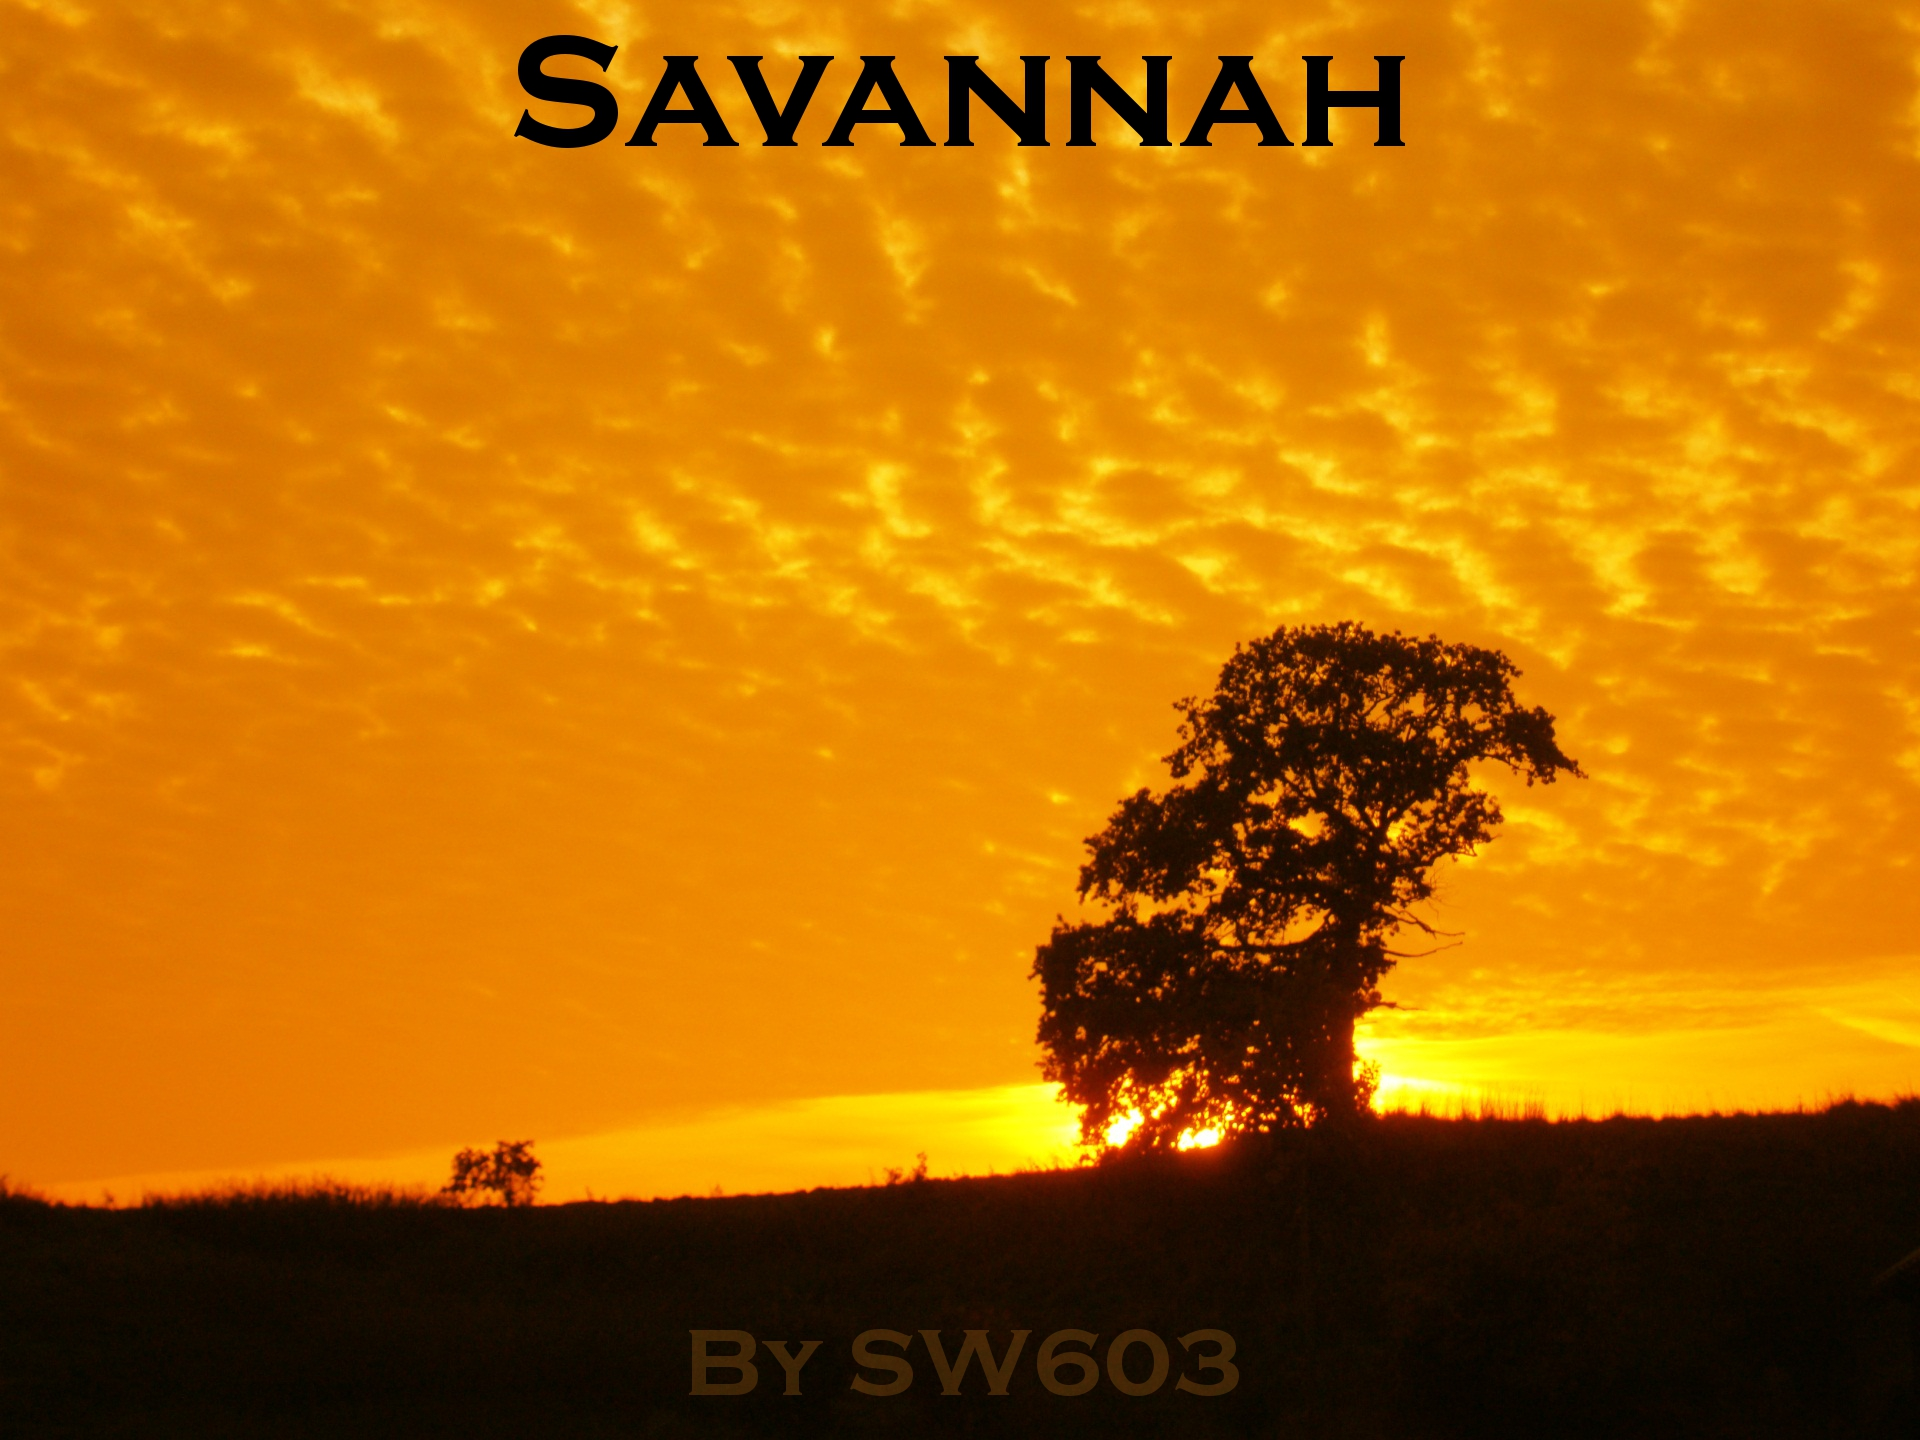
\includegraphics[width=1.00\textwidth]{Img/forside.jpg}
\end{figure}

\end{center}
\end{frame}
\begin{frame}
\titlepage
\end{frame}

\section{Intro}
\begin{frame}{Intro}
\pause
    \begin{block}{}
        \begin{itemize}
					\pause \item Pr�sentation af databasen
					\pause \item Pr�sentation af webinterface
					\pause \item Demo af webinterface
					\pause \item Pr�sentation af server
					\pause \item Demo af server
					\pause \item Udviklingsmetode
					\pause \item Konklusion
					\pause \item Sp�rgsm�l?
					\end{itemize}
    \end{block}
\end{frame}
\section{Requirements}
\begin{frame}{Requirements}
\pause
    \begin{block}{App groups}
        \begin{itemize}
					\pause \item Possibility to link pictures with sound
					\pause \item QR-code login for profiles
					\pause \item Ping functionality
					\pause \item Retrieval of either one profile, or children associated with specific guardians
					\pause \item Secure connection
				\end{itemize}
    \end{block}
\end{frame}
\begin{frame}{Requirements}
    \begin{block}{Customers}
        \begin{itemize}
					\pause \item Customizable software
					\pause \item That's it!
				\end{itemize}
    \end{block}
\end{frame}
\section{Database}
\begin{frame}{Database}
\pause
    \begin{block}{Requirements}
        \begin{itemize}
					\pause \item All users must be able to login with QR-code
					\pause \item All departments must be able to login
					\pause \item All users must be linked to at least one department
					\pause \item All guardians must be able to be linked to at least one child
					\pause \item All parents must be able to be linked to at least one child
					\pause \item All users must be able to access their selected apps
					\pause \item All users must be able to access their own pictures, and all public pictures
				\end{itemize}
    \end{block}
\end{frame}
\begin{frame}{Database}
    \begin{block}{Requirements continued}
        \begin{itemize}
					\pause \item All departments must be able to access all public pictures
					\pause \item All pictures needs to be able to be linked with tags.
					\pause \item All pictures must be able to be linked with audio and vice versa
					\pause \item All department must be able to have a subdepartment
				\end{itemize}
    \end{block}
\end{frame}

\section{ - Solutions}
\begin{frame}{Database - Requirements}
    \begin{block}{Solution}
					All departments must be able to access all public pictures
					
\begin{figure}[h]
	\centering
		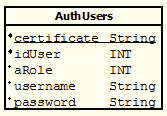
\includegraphics{Img/DatabaseQR.png}
\end{figure}

    \end{block}
\end{frame}

\begin{frame}{Database - Requirements}
    \begin{block}{Solution}
					All departments must be able to login

\begin{figure}[h]
	\centering
		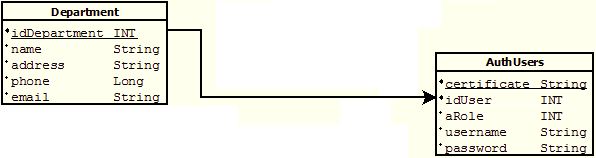
\includegraphics[width=1.00\textwidth]{Img/DatabaseDept.png}
	\label{fig:DatabaseDept}
\end{figure}
   \end{block}
\end{frame}

\begin{frame}{Database - Requirements}
    \begin{block}{Solution}
					All users must be linked to at least one department

\begin{figure}[h]
	\centering
		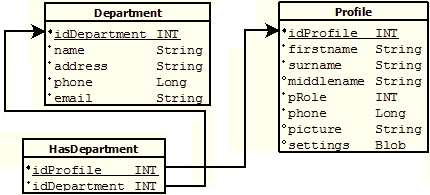
\includegraphics[width=1.00\textwidth]{Img/DatabaseProfileDeptRelation.png}
\end{figure}

   \end{block}
\end{frame}

\begin{frame}{Database - Requirements}
    \begin{block}{Solution}
					All guardians must be able to be linked to at least one child\\
					All parents must be able to be linked to at least one child

\begin{figure}[h]
	\centering
		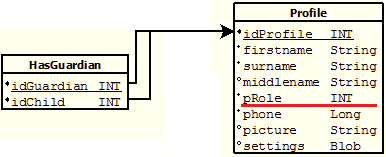
\includegraphics[width=1.00\textwidth]{Img/DatabaseProfileRoleLink.png}
\end{figure}

   \end{block}
\end{frame}


\begin{frame}{Database - Requirements}
    \begin{block}{Solution}
	All users must be able to access their selected apps
\begin{figure}[h]
	\centering
		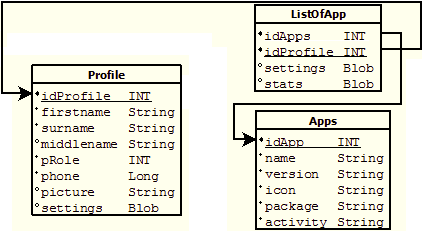
\includegraphics[width=1.00\textwidth]{Img/DatabaseProfileAppRelation.png}
\end{figure}

   \end{block}
\end{frame}

\begin{frame}{Database - Requirements}
    \begin{block}{Solution}
	All users must be able to access their own pictures, and all public pictures

\begin{figure}[htbp]
	\centering
		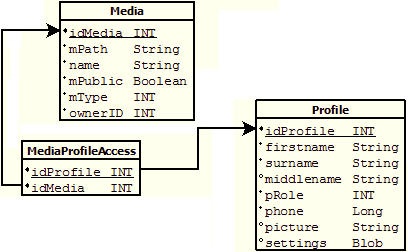
\includegraphics[width=1.00\textwidth]{Img/DatabaseProfileMediaRelation.png}
	\label{fig:DatabaseProfileMediaRelation}
\end{figure}

   \end{block}
\end{frame}

\begin{frame}{Database - Requirements}
    \begin{block}{Solution}
	All pictures needs to be able to be linked with tags.

\begin{figure}[htbp]
	\centering
		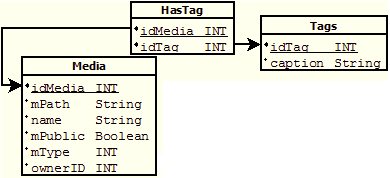
\includegraphics[width=1.00\textwidth]{Img/DatabaseMediaTagRelation.png}
	\label{fig:DatabaseMediaTagRelation}
\end{figure}

   \end{block}
\end{frame}

\begin{frame}{Database - Requirements}
    \begin{block}{Solution}
	All pictures must be able to be linked with audio and vice versa

\begin{figure}[htbp]
	\centering
		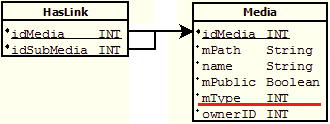
\includegraphics[width=1.00\textwidth]{Img/DatabaseMediaMediaRelation.png}
	\label{fig:DatabaseMediaMediaRelation}
\end{figure}

   \end{block}
\end{frame}

\begin{frame}{Database - Requirements}
    \begin{block}{Solution}
	All department must be able to have a subdepartment

\begin{figure}[htbp]
	\centering
		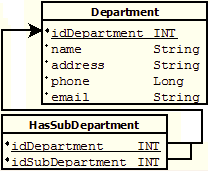
\includegraphics{Img/DatabaseDeptDeptRelation.png}
	\label{fig:DatabaseDeptDeptRelation}
\end{figure}

   \end{block}
\end{frame}

\section{ - Final design}
\begin{frame}{Database - Final design}
\begin{figure}[htbp]
	\centering
		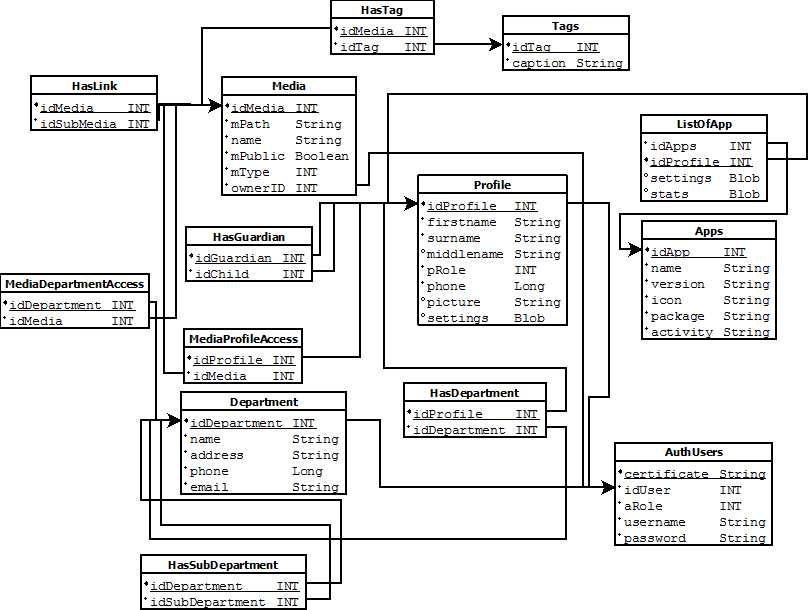
\includegraphics[width=1.00\textwidth]{Img/DiaDesign.png}
	\label{fig:DiaDesign}
\end{figure}


\end{frame}

\section{ - Testing}
\begin{frame}{Database - Testing}

    \begin{block}{Testing}
        \begin{itemize}
        \item Dynamic whiteboxing
        \item \pause Test-to-pass and test-to-fail
        \item \pause Went as expected!
				\end{itemize}
    \end{block}

\end{frame}
\section{Web-interface}
\begin{frame}{Web-interface}
\pause
		\begin{block}{Use Case}
				\begin{itemize}
					\item Karen Tailor Smith is an educator at Egebakken. She wants to create her own profile in the system. She wants her user name to be KTS and her password to be oliver (the name of her son).
					\item She then wants to create a profile for one of the children at Egebakken. The child's name is Eric Carter, she chooses his user name to be ``Eric C'' with the password ``EC''. He should have access to TestAppe1, which is an app on the GIRAF system. She then sets herself as his guardian.
					\item Karen realizes that she wrote the wrong phone number for Eric and wants to change it.
					\item When the summer comes, Eric is done at Egebakken, so Karen wants to delete his profile.
				\end{itemize}
		\end{block}
\end{frame}
\begin{frame}{Server Implementation}
  

\end{frame}

\section{Questions}
\begin{frame}

    \begin{block}{}
			
\begin{center}
Questions?
\end{center}
    \end{block}
\end{frame}

\end{document}